\documentclass[12pt]{article}
\usepackage{fontspec}
\usepackage{xeCJK}
\usepackage{minted}
\usepackage{xcolor}
\usepackage[a4paper, margin=2cm]{geometry}
\usepackage{setspace}
\usepackage{indentfirst}
\usepackage{tcolorbox}
\usepackage{graphicx}
\usepackage[stable]{footmisc}
\usepackage{hyperref}
\usepackage{csvsimple}

\hypersetup{
    colorlinks=true,
    linkcolor=blue,
    filecolor=magenta,      
    urlcolor=cyan,
}
 
\urlstyle{same}

\graphicspath{ {./images/} }

\onehalfspacing
\definecolor{friendlybg}{HTML}{f0f0f0}

\setCJKmainfont{Noto Serif CJK SC}
\setCJKmonofont{Noto Sans CJK SC}
\setromanfont{Noto Serif Regular}
\setsansfont{Noto Sans Regular}
\setmonofont{Fira Code}[
  Contextuals=Alternate  % Activate the calt feature
]
\usepackage{listings}
\usepackage{lstfiracode}

\definecolor{friendlybg}{HTML}{f0f0f0}
\ActivateVerbatimLigatures

\title{Make You a RISC-V Simulator}
\author{Alex Chi}
\date{July, 2019}

\newenvironment{aside}[1]
    { \begin{tcolorbox}[enlarge top by=0.5cm, enlarge bottom by=0.5cm] Aside\space\space\space\space \textbf{#1} \\
        } { \end{tcolorbox} }
        
\renewcommand{\figurename}{图}

\begin{document}

\maketitle 

    在过去的两个星期里,我用 C++ 实现了一个 RISC-V 模拟器。模拟器支持 RV32I 指令集。
    我先后完成了串行 (Sequential)、并行 (Pipelined) 以及乱序执行 (Out-of-order Execution)
    的模拟器。本文将介绍实现的细节和过程。

    \section{电路、FP 与串行模拟器}
    
    在设计之初,我希望模拟器的实现可以尽可能贴近硬件电路。其中的每一个操作,都是
    能够通过电路方便实现的。

    \begin{aside}{什么样的实现是贴近电路的?}
        电路不受外界条件影响,在寄存器的值和内存给定的情况下,不论仿真多少次,
        都能得到同一个值 (pure)。电路中也不宜设计一些复杂的数据结构(比如队列)。
        为了达成这个目标,我设计了第 \ref{register_model}
        章所述的寄存器类,并且在编程的时候增加了几个限制,这一部分参见第 
        \ref{feed_forward_evaluation} 章。
    \end{aside}

    在 CSAPP HCL 的启发下,我从函数式编程的角度考虑电路仿真,从而
    实现一个尽可能贴近硬件实现的模拟器。

    \begin{aside}{一个 CSAPP HCL 的样例}
        \begin{verbatim}
int dstE = [
    icode in { IRRMOVL } : rB; 
    icode in { IIRMOVL, IOPL} : rB; 
    icode in { IPUSHL, IPOPL, ICALL, IRET } : RESP; 
    : RNONE;
];
        \end{verbatim}
    \end{aside}

    \subsection{如何求解电路}

    \begin{figure}[h]
        \centering
        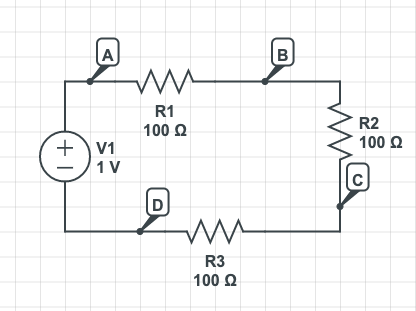
\includegraphics[width=0.5\textwidth]{circuit}
        \caption{一个电路}
        \label{fig:circuit}
    \end{figure}

    如图 \ref{fig:circuit} 所示,若要求得节点 C 处的电压,则必要先依次求出 A、B 处的电压。
    而当初始条件确定(电压源确定)时,不论求多少次 C 处电压,它永远都是一个值。由此,我联想到
    某个语言中的惰性求值 (Lazy Evaluation)。

    \begin{verbatim}
v_source = 1.0
current = 0.003333333
voltage_at_c :: Double
voltage_at_b :: Double
voltage_at_a :: Double
voltage_at_c = voltage_at_b - 100 * current
voltage_at_b = voltage_at_a - 100 * current
voltage_at_a = v_source

ghci> voltage_at_c
0.33333339999999995
    \end{verbatim}

    在 Haskell 中,我们可以描述函数之间的关系。在定义函数的时候,这些值都不会被立刻求出来。只有
    值被用到的时候,ghc 才会开始执行函数内容求值。这一思想可以被应用在电路仿真中。

    \subsection{如何设计电路}\label{feed_forward_evaluation}

    在 CPU 电路中,我们大体可以把元件分为两大类:时间控制和非时间控制元件。

    时间控制的元件包括寄存器、内存等。只有时钟发出信号,它们的值才会被更新,输出端的电平
    才会有变化。这些元件决定了电路的初始条件,是电路的信号源。非时间控制的元件包括各种选择
    器、运算器。这些元件端口的输出值可以通过信号源的电平决定。一旦电路达到稳态,它们的电平
    就不会再改变。

    因而,我们可以在程序中描述一组电路中的关系,就像之前的 Haskell 代码一样。而后,再用
    C++ 求得电路电平的关系,更新寄存器,开始下一个周期。

    设计电路的原则之一是:数据向前传播。在同一个周期内,这些电路元件之间的求值关系不应该出现
    互相依赖的关系。对于图 \ref{fig:circuit} 的电路,我们也可以用下面这段代码描述。

    \begin{verbatim}
voltage_at_c = voltage_at_b - 100 * current
voltage_at_b = voltage_at_c + 100 * current
    \end{verbatim}

    但这种描述就存在数据间的依赖关系。在设计 CPU 电路时,我们应当保证数据是单向传输的,对于
    每一根导线,我们可以人为规定它数据传播的方向(从寄存器输出到另一个寄存器输入)。在这一
    限制下,一个时钟周期内电路总能达到稳态。

    \subsection{寄存器模型}\label{register_model}

    \begin{figure}[h]
        \centering
        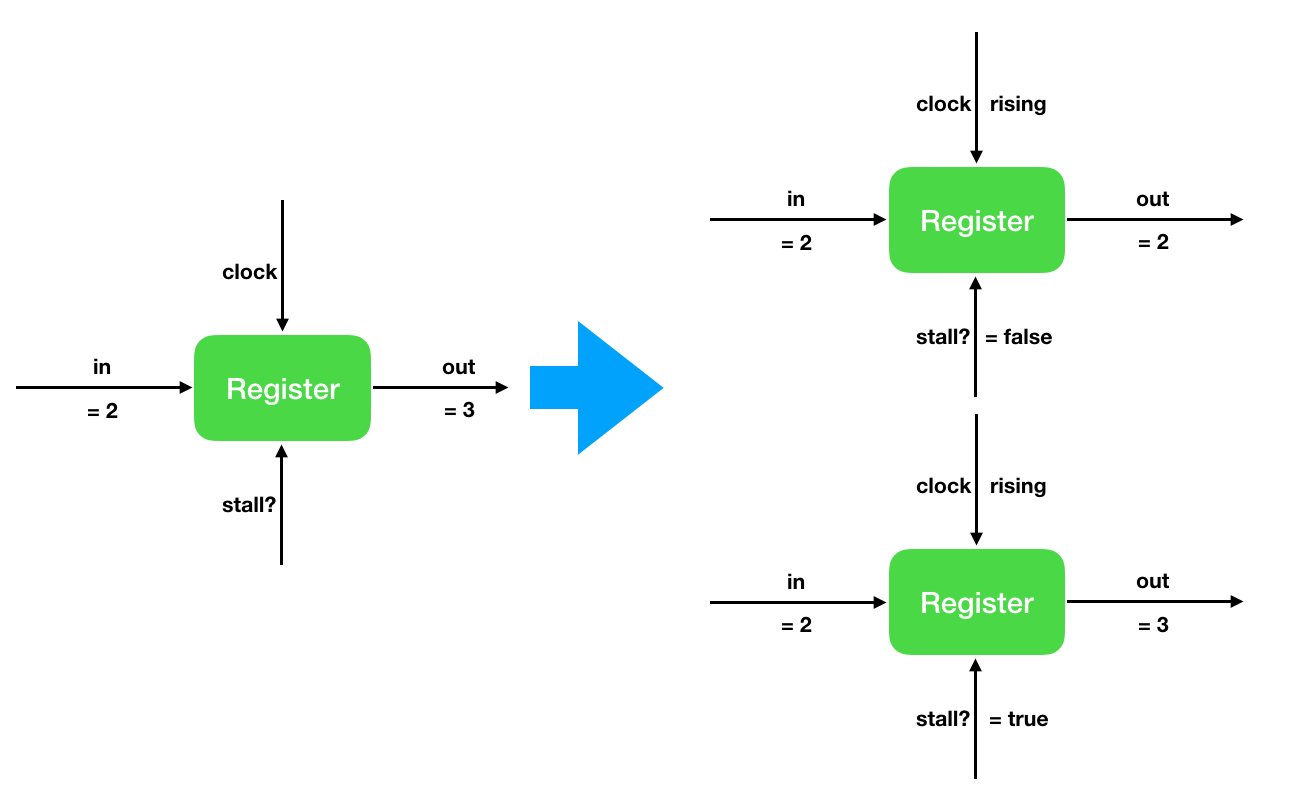
\includegraphics[width=0.8\textwidth]{register}
        \caption{寄存器模型}
        \label{fig:register}
    \end{figure}

    如图 \ref{fig:register} 所示,寄存器有一个数据输入端和一个数据输出端。寄存器由时钟
    控制。收到时钟信号 (tick),如果数据不被搁置 (stall),就将输出端设置为输入端的值。这一模型
    可以由下面的 C++ 代码所描述。

    \begin{verbatim}
template<typename T>
class Register {
public:
    T prev, next;
    bool _stall;
    Register() : prev((T) 0), next((T) 0), _stall(false) {}
    T read() { return prev; }
    T current() { return next; }
    void write(const T &t) { next = t; }
    void tick() { if (!_stall) prev = next; }
    void stall(bool stall) { _stall = stall; }
};
    \end{verbatim}
    \begin{tcolorbox}
        在第 \ref{new_register_design} 章中,我将会介绍一种可读性更高
        的寄存器类设计。
    \end{tcolorbox}

    \subsection{惰性求值在 C++ 中的实现}

    对于 CPU 中的每一个电路端口,我都确定了一个唯一的标签。通过标签即可得到端口的数据。
    比如,如果我们要在 Write-back 阶段完成 load 指令,将内存读取的值写入寄存器:
    \begin{verbatim}
// 获取寄存器写入目标
auto rd = session->d->get(Decode::rd);
// 获取内存阶段读到的值
auto m_val = session->m->get(MemoryAccess::m_val);
// 写入寄存器
session->rf.write(rd, m_val);
    \end{verbatim}

    在 Memory Access 阶段,我们定义求 \texttt{m\_val} 的方式。

    \begin{verbatim}
unsigned int addr = session->e->get(Execute::e_val);
switch (session->d->get(Decode::funct3)) {
    case 0b000: // LB
        return (char) session->memory[addr];
    case 0b001: // LH
        return (short) session->memory.read_ushort(addr);
    ...
}
    \end{verbatim}

    求 \texttt{m\_val} 的过程还会自动求 Execute 阶段所计算的内存地址。
    因此,通过惰性求值,程序能自动解决电路元件间的依赖关系。

    与此同时,由于一个时钟周期中,每个端口的值不论求多少遍都是一样的,我们可以通过 map
    或者其他方式将该周期里求过的端口值保存下来。在这个实现中,每个阶段的端口都由一个枚举类型
    定义。枚举类型的元素是一个从 0 开始编号的整型数。因此,我们可以直接用数组缓存端口的值。
    
    \begin{aside}{用 CLion 管理工程}
        在很久以前(大概是四年前),我对 CMake 最头大的事情是它没法用一条指令
        直接把整个目录的源文件都一起编译。在更久以前(大概是五年前),我对 C++
        最头痛的事情就是写它就要把声明与定义分离。把定义和实现拷来拷去,是一件令
        人头大的事情。后来,我发现了 CLion。我沉迷一键生成定义 (Definition),
        自动加载 CMakeLists.txt。自此以后,写 C++ 变成了一件不那么麻烦的事情。
        后来,随着 vcpkg 这类靠谱的 C++ 包管理器的出现,在 CMakeLists 中增加
        依赖也变得简单了许多。在这个项目中我就用到了 vcpkg 安装的 gtest。
    \end{aside}

    \subsection{串行模拟器的实现\protect
        \footnote{串行模拟器的实现在 seq 分支。
        \url{https://github.com/skyzh/RISCV-Simulator/tree/seq}}}

    在串行的 RISC-V CPU 中,电路中的时间控制元件只有内存、32 个寄存器和 PC。每个时钟周期中,
    各个电路元件从 PC 开始依次读出指令、获取操作数、执行计算、写内存、写寄存器,并将新的 PC
    写入 PC 寄存器中。写入寄存器的数据在这一个时钟周期中无法被读出。在数据更新完成后,对所有
    时间控制元件执行``tick''操作,开始下一个时钟周期后,这些写入的数据才能被电路元件读取到。

    \begin{aside}{一些常见的坑}
        第 0 个寄存器永远是 0。
        
        \texttt{JAL}、\texttt{JALR} 指令要把 \texttt{PC + 4} 写入 \texttt{rd}。
    \end{aside}

    因而,从程序模拟的角度来说,我们只需要求得电路输出的值就可以完成一个周期的模拟。在串行 CPU
    中,整个电路有三个输出:到 PC 寄存器的输出,向内存写入,以及向 32 个寄存器写入。这就是每次
    更新所需要做的事情。

    \begin{verbatim}
PC.write(w->get(WriteBack::w_pc)); // 更新 PC 寄存器
m->hook();                         // 写入内存
w->hook();                         // 写入寄存器
    \end{verbatim}

    由于我们在程序中通过函数的调用关系确定了求值顺序,三句语句可以任意调换而不影响最后的结果。

    \begin{aside}{写点单元测试}
        在完成 PPCA 的几个项目的过程中,我用 Google Test 写了一些单元测试。虽然单元测试通过
        并不能保证整个程序可以跑起来,甚至单元测试也没法覆盖所有样例,但如果单元测试挂了,那必然
        是改程序改错了。比如在写 Parser 的过程中,我发现有些时候内存里读到的指令是 
        \texttt{0xffffffff}。于是,我加上了 hex dump 中行末有空格、有各种换行的 Parser
        单元测试,发现了问题所在。
    \end{aside}

    \section{更快的电路仿真:从串行到并行}

    在上一章中,我介绍了串行模拟器设计的过程和其中的一些问题。由于从项目一开始我就采用电路仿真
    的思路,所以从串行改并行的过程中,我几乎没有进行大的重构。但是后来我发现,惰性求值效率很低。
    因此,在这一章中,我提出了另外一个电路仿真的方法,并且验证了这种方法依然是 pure 的。
    
    在这一部分,我完成了一个通过数据转发 (Forwarding) 解决数据冲突 (Data Hazard) 的 CPU 模拟器。
    模拟器还采用了两位自适应分支预测 (Two-level Adaptive Predictor),在部分样例中达到了 98\% 的
    准确率。

    \subsection{手动指定求值顺序}

    \begin{verbatim}
w->hook(); // Write back
m->hook(); // Memory access
e->hook(); // Execute
d->hook(); // Decode
f->hook(); // Fetch
    \end{verbatim}

    比如,在 Decode 阶段,我们需要确定后面的阶段中是否有 Hazard。因而,Decode 阶段必然在 Write Back、Memory Access 和 Execute 阶段之后执行。

    以这样的求值顺序,只需要将不同阶段的 hook 调用一次,就可以达到电路稳态。这样,模拟器运行起来就更快了。

    \subsection{五级流水线设计与实现\protect
        \footnote{并行模拟器的实现在 pipeline 分支。
        \url{https://github.com/skyzh/RISCV-Simulator/tree/pipeline}}}

    \subsection{验证并行实现确实并行}

    在 Session.cpp 中随机选取五个阶段的求值顺序。这个循环执行十遍后,电路必然可以达到稳态,
    它和手动指定求值顺序的结果一致。因此,模拟器的运行和五个阶段的求值顺序无关。这个模拟器是并行的。
    验证的代码如下。

    \begin{verbatim}
int seq[5] = { 0 };
for (int j = 0; j < 5; j++) seq[j] = j;
for (int i = 0; i < 10; i++) {
    std::random_shuffle(seq, seq + 5);
    for (int j = 0; j < 5; j++)
        switch(seq[j]) {
            case 0: f->hook(); break;
            case 1: d->hook(); break;
            case 2: e->hook(); break;
            case 3: m->hook(); break;
            case 4: w->hook(); break;
        }
}
    \end{verbatim}

    当然也有其他方法验证。比如开五个线程分别更新五个阶段,每隔 1ms 更新一次时钟。这种验证方法
    似乎就更加贴近电路中电压的传播了。

    \begin{tcolorbox}
        理论上,我们也可以跑五个线程分别刷新五个阶段的电路。但事实是,这么做会导致
        各种异常。这可能是因为对寄存器的操作存在 data race。
    \end{tcolorbox}

    \subsection{模拟器使用的 CPU 电路}

    \begin{aside}{自己造数据}
        如果直接用现有的样例测试模拟器的正确性,似乎有些难度。因而,我通过 
        \href{https://github.com/TheThirdOne/rars}{RARS} 编写 RISC-V 汇编,
        造了几组测试数据,用于检查模拟器面对 Data Hazard 和
        Control Hazard 时的行为。这些测试样例都可以在 \texttt{tests/} 目录下找到。
    \end{aside}

    https://github.com/skyzh/RISCV-Simulator/files/3362948/RISCV.Design.pdf
    
    \subsection{分支预测}

    在完成五级流水线后,我开始探究分支预测的实现。原本的实现对于分支指令,一律预测紧接的一句
    (Always not taken)。对于 \texttt{JAL}、\texttt{JALR} 之类的指令,也在 Execute
    阶段才进行处理。在此基础上,我实现了两位自适应分支预测 (Two-level Adaptive Predictor)。
    
    \begin{tabular}{|l|c|c|c|c|}
        \hline
        \bfseries 数据 & \bfseries 预测前周期 & \bfseries 预测后周期 & \bfseries 周期减少率 & \bfseries 预测成功率
        \csvreader[head to column names]{tables/branch_prediction.csv}{}
        {\\\hline $\data$ & \beforecycles & \aftercycles & \cycleimprovement & \afterrate}
        \\\hline
    \end{tabular}

    \begin{aside}{使用 git 管理工程}
        说到分支,就不得不提 git 的分支(虽然此分支非彼分支)。在这个项目中,我通过 git 管理工程,开了许多分支。
        它们包括:seq (Sequential, 串行实现)、feedforward (手动指定求值顺序的串行实现)、pipeline (并行实现)、
        out-of-order (乱序实现)。我时常在不同分支间切换,以修改某个版本的 bug。偶尔也会在大改项目
        之后,再切换分支参考之前写过的代码。
    \end{aside}

    \section{基于 Tomasulo 算法的乱序执行}\label{out_of_order_execution}

    在乱序执行中,原有的五级流水线最后只剩下两个大部分:发布指令 (issue) 阶段和乱序执行
    (OoOExecute) 阶段。在乱序执行阶段中,原有 Execute 阶段的 ALU 变成了一个小单元,
    Memory Access 变成了 Load-Store 单元。

    由于我并不知道改如何设计基于 Tomasulo 算法的硬件,在这一章节中的程序仅仅是一个
    展现乱序执行的纯算法模拟。
    \footnote{乱序执行模拟器的实现在 out-of-order 分支。
        \url{https://github.com/skyzh/RISCV-Simulator/tree/out-of-order}}

    \subsection{新的寄存器类设计}\label{new_register_design}

    \begin{verbatim}
template<typename T>
class Register {
    ... // 这一部分和之前的 Register 类一致
    operator T() { return read(); }
    void operator=(T next) { write(next); }
};
    \end{verbatim}

    在这一设计下,整个程序的可读性将大大提高。比如在 Tomasulo 算法的放操作数阶段:

    \begin{verbatim}
void Issue::issue_rs_to_Vk(unsigned reg_id, RS *rs, RSID unit_id) {
    if (reg_id != 0 && session->e->should_rename_register(reg_id)) {
        rs->Vk = 0;
        rs->Qk = session->e->get_renamed_register(reg_id);
    } else {
        rs->Vk = session->rf.read(reg_id);
        rs->Qk = NONE;
    }
}
    \end{verbatim}

    在这里,\texttt{Vk}, \texttt{Qk} 都是寄存器。对 \texttt{Vk} 和 \texttt{Qk} 的
    操作,只有在下一个周期才会生效。因而,这种寄存器类的设计在不影响理解的同时,增加了
    代码的可读性。

    当然,在某些情况下,这种写法或许会让人有些误解。比如在发出指令阶段。

    \begin{verbatim}
pc = pc + 4
    \end{verbatim}

    在这里,我们把当前时钟周期 \texttt{PC} 读出,通过某个硬件单元加了 $4$,并把结果接回了
    \texttt{PC} 寄存器上。因而,在同一个时钟周期里,不论这句话被执行几次,下一周期的 \texttt{PC}
    永远是这一周期的 \texttt{PC} 加上 $4$。

    \subsection{仅基于 Tomasulo 算法的 CPU 设计}

    在 \emph{Computer Architecture: A Quantitative Approach} 的第 3.5 节中,作者介绍了
    Tomasulo 算法。但是在这一章节中,缺少很多实现的细节,以至于我无法直接参照书本实现一个 CPU。

    \subsection{RV32I 中较难处理的指令}

    在实现 Tomasulo 算法的过程中,我发现 RV32I 的部分指令需要多个硬件单元或者特殊处理才能完成。

    \texttt{JALR} 指令需要将指令中 \texttt{rs1 + imm} 计算出来作为跳转的目标,而后将
    \texttt{PC + 4} 存入 \texttt{rd} 之中。在 Tomasulo 算法的实现中,我将这一指令发送
    到两个计算单元。由 \texttt{BRANCH1} 计算 \texttt{rs1 + imm},并且用 \texttt{ADD1}
    计算 \texttt{PC + 4}。当 Issue 阶段发现这个指令时,流水暂停,直到 \texttt{BRANCH1} 计算出
    下一个指令的地址才继续发送指令。

    在后文第 \ref{hardware-speculation} 章中实现推测执行时,\texttt{JALR} 指令需要更加复杂
    的处理。由于使用了两个运算单元,它需要分配两个重排缓冲中的空位。两个空位中,第一个为 \texttt{ADD1}
    的输出,并且在向第一个空位发送指令的时候,将指令当作 \texttt{JAL} 处理。(\texttt{JAL} 指令
    在发出的时候就能确定跳转目标,在最后提交的时候就只需要把 \texttt{PC + 4} 存入 \texttt{rd},
    提交的过程和 \texttt{JALR} 拆分的第一个操作一致)。第二个操作和分支指令类似,只不过是无条件
    跳转。当提交 \texttt{JALR} 的第二个操作时,就相当于分支预测失败,要清除重排缓存。
    
    分支指令的实现也比较困难。我给分支指令分配了一个运算单元 \texttt{BRANCH1},它的功能和其他的 ALU
    单元一致。当发出分支指令时,流水线停止,将分支按照跳转方法转换为 ALU 可以处理的运算,并将运算结果
    存入新增的第 33 个寄存器中。当这个专用寄存器被写入、\texttt{BRANCH1} 运算单元空闲时,发出
    阶段就能确定下一条指令的位置。这个过程会导致大量的时钟周期浪费在处理分支上,流水线在处理分支的时候
    不能发出新的指令。这一问题也在后文第 \ref{hardware-speculation} 章中通过硬件推测解决了。


    \begin{aside}{调整 Debug 输出,或许会有好心情}
        在实现乱序执行的过程中,我时常要观赏一个时钟周期里的所有硬件数据,来判定问题发生的地方。
        这些数据包括:发出的指令、PC、寄存器的值、寄存器重命名情况、Reservation Station 的
        情况。一个 Cycle 的信息可以打一整屏幕。此时,对 Debug 输出排版就显得尤为重要。
        对于 32 个寄存器,我在调试信息中打出了它们的名字,并同时输出十进制值和十六进制值。
        对于正在处理数据 (busy) 的单元,我会用 Emoji 符号(比如红色的圈圈)突出显示。
    \end{aside}

    \subsection{推测执行与重排缓冲}\label{hardware-speculation}

    在完成基于 Tomasulo 算法的乱序执行后,根据 \emph{Computer Architecture: A Quantitative Approach}
    的介绍,我对设计进行改进,添加了重排缓冲 (Reorder Buffer),实现了推测执行 
    (Hardware Speculation)。

\end{document}
